\documentclass[letterpaper, 12pt]{article}
\usepackage{cmjStyle}
\usepackage{natbib}
\bibpunct{(}{)}{;}{a}{}{,}
\doublespacing
\raggedright
%\setlength{\parindent}{0} % first para indent?
\setlength{\parskip}{2ex}
\parindent 24pt
\urlstyle{same} % make url tags have the same font
\setcounter{secnumdepth}{-1}

%% The package endfloat moves all floats (figures, tables...) to the
%% end of the paper, as required for the final version of a CMJ paper.
%% Leave this package commented out for initial submission, but
%% uncomment it for final version.
% \usepackage{endfloat}

\begin{document}

%% %author - name
%% {\cmjAuthor Vilson Vieira, Renato Fabbri, Guilherme Lunhani, Geraldo Magela de Castro Rocha Junior}
%% %author - address
%% \newline
%% \begin{cmjAuthorAddress}
%%     Instituto de Física de São Carlos\\
%%     Universidade de São Paulo\\
%%     1234 Anywhere Street\\
%%     Anywhere, Anwhere 012345 USA\\
%%     vilson@void.cc, renato.fabbri@gmail.com, gcravista@gmail.com, gera.sp@gmail.com
%% \end{cmjAuthorAddress}

\vspace*{24pt}

%{\cmjAuthorPhone << AUTHOR TELEPHONE (not for publication): +55 16 8108 7007 >>}

 {\cmjTitle Vivace: A Collaborative Live Coding Language}

% outros títulos.. ??????????
% Vivace: Freak Coding on Your Face

\section*{Abstract}

In this paper we describe the principles and the design behind Vivace,
a live coding language built on Web. We start by reviewing what
motivated and inspired the creation of the language. It's
specification and how it is parsed and executed using the recently
created Web Audio API is then described. We discuss why the Web is an
interesting environment to collaborative live coding and how it
affected the performances. We conclude by previewing how Vivace is
motivating the creation of other live coding languages and new
artistic genres, like Freak Coding.

\section*{} % Introdução, sem título.

In November of 2011 a live coding trio called FooBarBaz performed
their first presentation for a wide audience~\footnote{Pictures of the
  presentation is available at
  \url{http://www.flickr.com/photos/festivalcontato/6436260557}}. Live
coding is becoming popular world wide but remains untouched in
Brazil. We believe that this presentation was the first live coding
performance in our country. In that day an audience of about 5000
attendees was introduced to an alternative audiovisual performance
where code was used to create the music they were listening and, at
same time, projected on two big screens.  

During the performance, the trio used ChucK~\cite{wang2003chuck} in an
uncommon way. Instead of writing loops and conditionals, they
manipulated parameters of audio samples files by editing lists of
numerical sequences. Mnemonic operations (e.g. reverse, retrograde,
transposition) were used on those sequences together with easy audio
mixing (originally done in Puredata) and skeletons of
code quick-inserted by editors. This revealed as good practices to
live code during the performance.  

Based on those elements we designed a new language to be used on the
subsequent sessions: Vivace~\footnote{Vivace source code is online at
  \url{http://automata.github.com/vivace}}. We wanted to avoid
software configuration and make it easy to share the session -- and
the code -- with everyone. Thus, the Web was choosen as the running
environment for Vivace. On every new session we performed using
Vivace, new principles were added into the language and, at the same
time, into our artistic behaviour.  

In summary, this paper is a circle: we describe how a performance
motivated the language and how the language influenced the creation a
our style to live code that we now call Freak Coding.

% DEPRECATED??:
%In summary, this paper describes:
%
%\begin{enumerate}
%  \item good artistic practices identified for live coding
%  \item language specs (Jison parsing a context-free grammar, DSL)
%  \item the audio engine (Web Audio api, Why web?)
%  \item the collaborative behavior (ShareJS and Web)
%  \item environment (the whole system + GUI)
%  \item uses and future work (easy input for broad audience using
%    the pad without breaking the session, a language focused on live
%    cinema, OSC/MIDI/web cam, 'freak coding' as live coding subgenre)
%\end{enumerate}

\parskip 18pt

\section{Motivation \& inspiration: arrange the room, the code is dirty}

Vivace is inspired by couple of live coding languages. The sintax of Vivace, as shown in Figure~\ref{fig:vivace}, borrows elements from ixi lang~\cite{magnusson2011ixi} like the use of sequences as audio parameters. ABT (REF) was strongly important to the development of Vivace as well and we are planning to rewrite some of its components -- originally in Python -- inside Vivace. From ChucK we used the concept of chained unit generators specified by the $=>$ operator, imitating the objects connections in visual programming languages like Puredata.

\begin{figure}[htpb]
\begin{center}
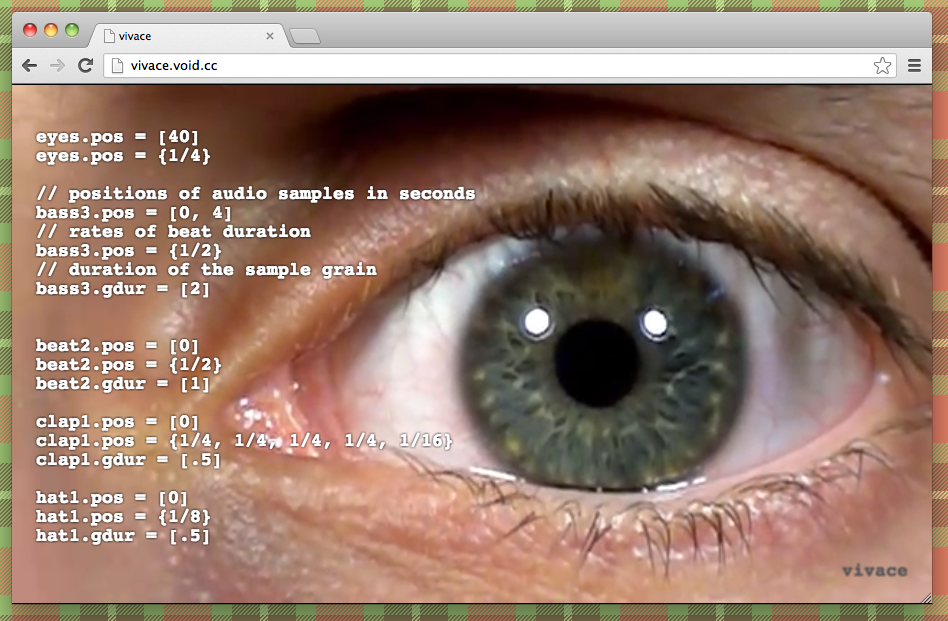
\includegraphics[scale=.3]{img/fig_vivace.png}
\caption{The Vivace environment}
\label{fig:vivace}
\end{center}
\end{figure}

Along these \textit{desktop languages}, Vivace was also inspired by
Web live coding languages. After the creation of Audio Data API and
the most recent Web Audio API~\cite{webaudio} -- that makes possible
to process audio in real time inside Web browsers -- a collection of
audio Web applications started to emerge. The same was true for live
coding languages and systems. Vivace is part of this \textit{family}
of Web applications together with Gibber~\cite{gibber},
livecoder~\cite{livecoder}, livecoding.io~\cite{livecodingio} and
livecodelab~\cite{livecodelab}, to note some of them. A remarkable
difference between Vivace and those languages or environments is the
collaborativity. Vivace was built to make possible to write code with
many hands at the same time, using the now popular "pads" -- a
characteristic easily implemented on Web but not so much on desktop
languages. Another difference is the unconcern to be a Turing-complete
language, that made the design of Vivace more flexible and near of the
music process instead of the computing process (a characteristic that
we got from ixi lang). Vivace tries to balance between the rigorous of
code and the flexibility of artistic expression.

\section{The language We all Speak}

Vivace, as a language\footnote{The complete language specification is
  online at
  \url{https://github.com/automata/vivace/wiki/Language-spec}}, is a
collaborative livecoding language with use of extreme simple language
sintax, mnemonic actions, easy mixing, template editing and audio
parameters automation. In our experiences, the use of a shared code,
sounds and images leads a more complex experience, thus greater the
possibility of inconsistency of compiled code as well as actions for
artistic result, leading us to discriminate specific language
syntaxes.  

As already discussed, the language borrows elements from several
computer music languages and systems, like ixi lang and ABT. It is not
an imperative language. Instead of routines and procedures modifying
the audio voices, we used definitions. The motivation behind the use
of definitions is related with musical scores and the \emph{track
  paradigm} used on music production softwares. It is more familiar to
musicians (and, as we experienced on performances, to non-musician
people) to understand a sequence of notes, or audio parameters, than a
for-loop and if-chains. In this way, Vivace is a declarative, domain
specific language, based on the following principles:

\begin{itemize}
  
\item Names are something like $a$, $b$, $c$ and are dinamically defined.
\item Music is made by voices (instruments).
\item Voices have name, timbre and parameters ranging along the
  time.  \item The language should be simple. ``Freak Coders''
  (\ref{freakcoding}) only define some properties with a set of values
  (i.e. arrays, dictionaries) making possible to generate sequences,
  even using list comprehension.
\item Use mnemonic music-like operations (reverse, inverse, transpose)
  on these properties with syntax sugar (with care): few chars, big
  results
\item Timbre are signals made by chains of audio generators and
  filters or video files as described in Section~\ref{audioengine}
\item Parameters are musical notes, amplitudes, oscillators frequency,
  delay time and so on.
\item Parameters changes their values at some time and have some
  durations.

\end{itemize}

Here is a ``Hello, World!'' listing. A voice is defined as \textit{foo} and its parameters are specified using the \textit{dot} operator. Every parameter changes overtime assuming the values written as sequences surrounded by brackets. An special sequence exists to every parameter. They are used to specify the time durations of each parameter value and are surrounded by keys instead. This is all the Vivace syntax.

\begin{Verbatim}[fontfamily=courier, xleftmargin=\parindent]
  # foo is a simple audio sample, oscillator or video file
  foo.src = youtube('http://www.youtube.com/watch?v=XXX')
  # defining the video positions (in seconds) to be played
  foo.pos = [10, 20, 35]
  # the durations (as time ratios) to play each position
  foo.pos = {1/2, 1/4, 1/8, 1/16, 1}
\end{Verbatim}

There is extra semantics to operate on the typed sequences. Every
sequence accepts operators: mnemonic commands used to reverse,
transpose and even replace elements of the sequence based on list
comprehensions. Those operations are common in music composition and
having them as mnemonics makes typing fast and handy for live
coding. The next listing shows them.

\begin{Verbatim}[fontfamily=courier, xleftmargin=\parindent]
# we can use operators

foo.pos = [1, 2, 3] reverse        # result is [3, 2, 1]
foo.pos = [1, 2, 3] inverse        # result is [1, 0, -1]
foo.pos = [1, 2, 3] transpose +2   # result is [3, 4, 5]

# and even list comprehension

foo.pos = [1/i+1 for i in [1, 2, 3]] # result is [2, 3, 4]

# or combine both

foo.pos = [1/i+1 for i in [1, 2, 3]] reverse 

# result is [4, 3, 2] as spected
\end{Verbatim}

Vivace is written in JavaScript to take advantage of Web technologies.
To parse Vivace we used Jison~\cite{jison}, a JavaScript library that
clones Flex and Bison functionalities as lexer and parser. This
flexibility to parse and execute new languages as JavaScript inside
every browser opens an oportunity to experiment with new sintaxes and
semantics. And considering that Web was always strong on UI
development thanks to HTML and CSS, we can experiment those new
languages with fast prototyped UI. Along thise advantages, another one
is remarkable: every live coding language built on Web runs everywhere
a browser is present. No firewall chain, no software installation and
configuration, no dependencies, people just need to type an URL.

\section{The Audio Engine}
\label{audioengine}

Before Web Audio API, the only way to create sound in web pages was
using plugins. Recently, Web Audio API makes possible to do audio
processing in real time on Web browsers (as this paper was written,
only Google Chrome and Apple Safari supported the API and Mozilla is
working to have it running on Firefox as well). Every routine is
writen as native code (in C++ and Assembly) to guarantee
performance. The API is based on a convenient paradigm: audio unit
graphs. In this way, it specified a collection of nodes (AudioNode
objects) and routines to connect and disconnect them. While
manipulating those nodes we can create a large number of audio
synthesizers, filters, analysers, mixers and so on. This motivated us
to explore a basic approach of multichannel expansion, filtering and
audio effects (like languages as SuperCollider, Puredata), controling
an integrated Web audio system.

Every voice in Vivace is represented as an standard audio chain
(Figure~\ref{fig:chain}). All audio units parameters within this chain
could be manipulated editing the code or by sliders on a UI
(Fig.~\ref{fig:ui}). This kind of interface is more familiar to
musicians (remembering a real mixer) and makes possible an adequate
treatment of voices timbre and spacial sensations of the sound sources
(parameters like the level of stereophonics channels L and R, 3-band
equalization filters and reverb time control).

\begin{figure}[htpb]
  \begin{center}
    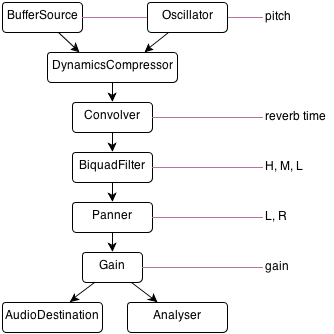
\includegraphics[scale=.5]{img/fig_chain.png}
    \caption{Standard audio units chains as Web Audio API objects for
      each Vivace voice.}
    \label{fig:chain}
  \end{center}
\end{figure}

\begin{figure}[htpb]
  \begin{center}
    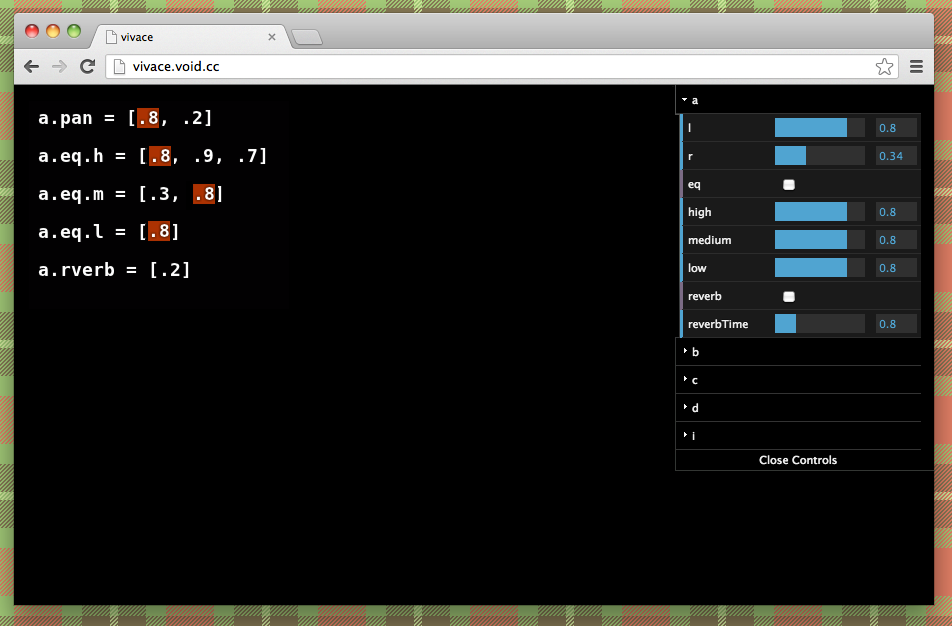
\includegraphics[scale=.3]{img/fig_ui.png}
    \caption{Every audio unit parameter can be manipulated by code or
      using the UI.}
    \label{fig:ui}
  \end{center}
\end{figure}

\section{Into the wild: making it collaborative}
\label{freakcoding}

Vivace as a tool makes possible interaction while everyone could use
its own creativity. The interaction is not more the same on classical
music, mediated by a common score, but by a mutual desire. With this
freedom we can create a composition in real time. In this context
borns the Freak Coder (Figure~\ref{fig:freakcoder}): someone that adds
up his individuality to others aiming to transform the computer in an
instrument of artistic fruition without restricting to itself the
machine control but opening and inviting everytone to do the
same. Freak Coder decides what he is going to do, amplifies his own
comprehension of computer capacity as an instrument. By using simple
rules, Vivace makes the emergence of the performance and makes it a
kind of collective game where the rules, being visible to everyone,
makes easy to them join in this game.

\begin{figure}[htpb]
  \begin{center}
    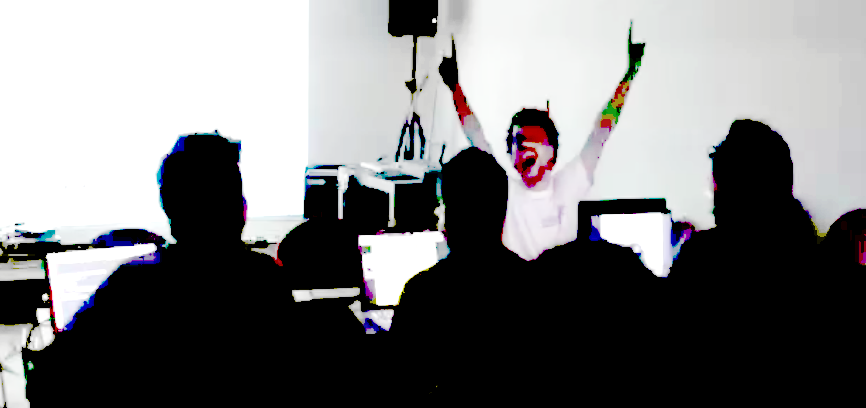
\includegraphics[scale=.4]{img/fig_freakcoder.png}
    \caption{Freak Coder}
    \label{fig:freakcoder}
  \end{center}
\end{figure}

Live Coding becomes a natural path to the type of use and
technological development in which we are already envolved, coming
from the principle that we understand that technology never should be
treated as dogma or secret. The Live Coding is a disalienation of the
behavior of a digital artist. Not only the code is showed and
manipulated, but the computer screen and any interaction between the
performance and the computer. The triad performancer, computer and
audience together makes possible to call the performance Live
Coding. The simple existence of a big screen with images passing on
it, no.  

This comprehension was possible after a presentation by LabMacambira
at the 9th edition of AVAV (\textit{\'{A}udio Visual Ao Vivo} or Live
Audio Visual) an event where artists who are experimenting audio and
video in real time comes together to show their works. In this
presentation...

%O Vivace como ferramente possibilita que aja interação, permitindo a
%cada um usar sua critividade. A interação não se dá mais a partir de
%uma partitura em comum, mas através de um desejo mútuo. Essa
%liberdade possibilita uma obra que se dá no tempo real. É nesse
%contexto que nasce o Freak Coder, um sujeito que soma sua
%individualidade a de outros para transformar o computador em um
%instrumento de fruição artistica sem restringir para si o controle
%sobre a máquina, mas abrindo e convidando a todos a fazerem o
%mesmo. O Freak Coder decide o que irá realizar, amplia a própria
%compreenção da capacidade do computador como instrumento.

%Por se utilizar de regras simples o Vivace permite a emergêrcia do
%resultado da performance e coloca como uma forma de jogo coletivo no
%qual as regras por estarem visivéis a todos permite uma rápida
%entrada nele.

\begin{figure}[htpb]
  \begin{center}
    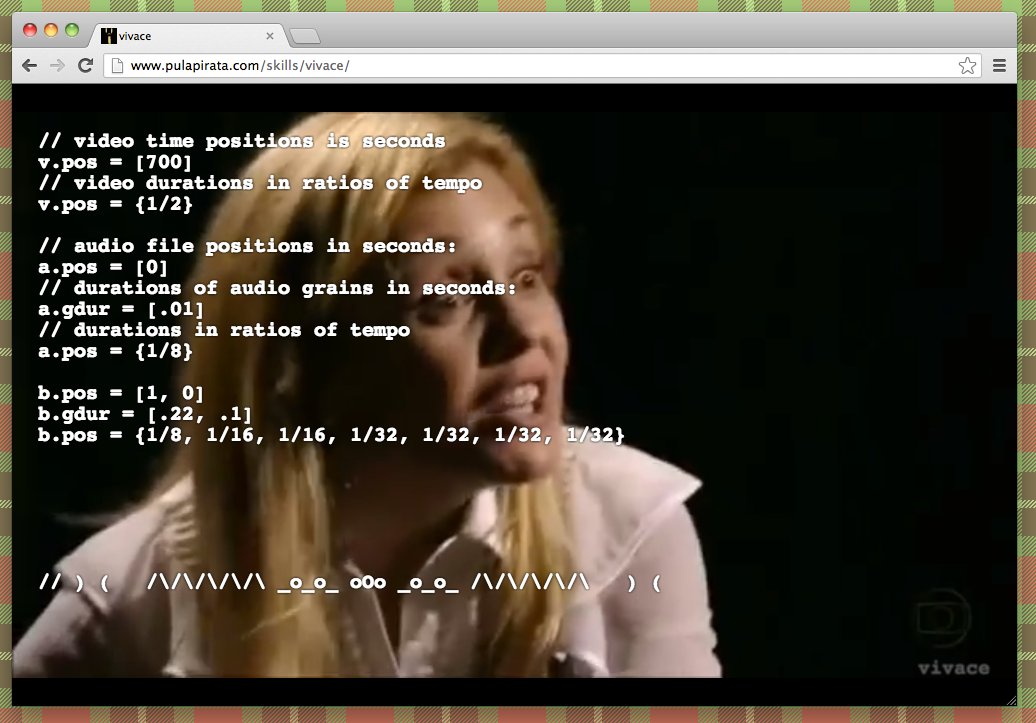
\includegraphics[scale=.3]{img/fig_novela.png}
    \caption{Videos from popular Brazilian novels were used as
      material: extreme pop-art.}
    \label{fig:novela}
  \end{center}
\end{figure}

%O Live Coding torna-se um caminho bastante natural para o tipo de
%utilização e desenvolvimento tecnológicos no qual já estamos
%envolvidos, partindo do principio de que entendemos que a tecnologia
%nunca deve ser tratada como dogma ou segredo. O Live Coding aparece
%cada vez mais como uma desreificação do fazer artístico digital. Não
%apenas o código é mostrado e manipulado, mas, sim, a tela do
%computador e qualquer interação que houver entre o performer e o
%computador. A tríade performer, computador, público é o que
%possibilita dizer que algo é uma performance de Live Code. A
%existência de um telão passando imagens, não.

%Essa compreensão se deu em grande parte depois da apresentação
%realizada pelo Lab Macambira no AVAV 9 (Áudio Visual Ao Vivo, Nona
%edição), evento no qual artistas que estão experimentando áudio e
%vídeo em tempo real se reunem e mostram seus trabalhos. Nesta
%apresentação estavam Caleb Luporini, Gera Rocha, Renato Fabbri e
%Vilson Vieira. Como Renato Fabbri e Vilson Vieira estavam vindo de
%São Carlos, Caleb Luporini e Gera Rocha começaram a apresentação sem
%que os outros dois integrantes tivessem chegado. Quando ambos
%chegaram ligaram seus computadores e passaram a interferir na
%performance através do Vivace sem que isso trouxesse nenhuma forma de
%constrangimento ou ruptura acontecesse na apresentação. É importante
%ressaltar que mesmo entre Caleb Luporini e Gera Rocha não havia
%acontecido qualquer tipo de ensaio ou combinados, sendo que os
%próprios vídeos escolhidos para a apresentação haviam sido escolhidos
%por Caleb e os outros integrantes não tinham visto ele ainda. No
%decorrer dos 30 minutos de apresentação pessoas que estavam no papel
%de platéia e seguindo as orientações que estavam na interface do
%Vivace passaram a acessá-lo e editar junto com os performers.

%Outra característica que emergiu dessa apresentação foi a capacidade
%de mesmo em um ambiente 'formal' de apresentação - os quatro
%performers estavam em uma sala escura, três virados para o telão e um
%virado para o público, que estava em cadeiras organizadas como em um
%teatro - gerar um estado de euforia coletiva. É importante a reflexão
%sobre como a soma entre máquina e humano gera esse estado. É a
%postura do performer diante do computador que tira aquele que deveria
%apenas assitir desse lugar e possibilita que uma experiência que é
%altamente técnica no que se refere ao desenvolvimento tecnologico do
%qual é origem tornne-se assimilável e lúdica. Durante toda a
%apresentação todos os integrantes do Lab Macambira riam entre si e
%estabeleciam uma relação com o público que era de leveza e
%fraternidade, isto é, o público era constantemente convidado pela
%postura do Lab Macambira a interagir com o que estava sendo proposto
%ali. Essa troca entre os quatro elementos ali presentes - performers,
%computador, Vivace, público - são capazes de criar um ambiente de
%colaboração e liberdade geradores de ludicidade e conhecimento
%realmente inéditos, pelo menos no que se refere a Live Code feito no
%Brasil. É, como explicado acima, a esse 'facilitador' que emergiu que
%passamos a chamar de Freak Coder.

%Todos integrantes do Lab Macambira são originários dos movimentos de
%software livre brasileiros. E é aí onde primeiramente devemos buscar
%pistas da origem do Freak Coder, que um programa com as
%características do Vivace possibilitou emergir. É totalmente inerente
%ao movimento do software livre a transmissão continua daquilo que se
%sabe. Assim como a desmistificação da tecnologia e o comportamento
%festivo e gregário.

%No ponto performer/computador é onde esse devir se concretiza. Mais
%do que o conteúdo utilizado no Live Coding a postura do performer em
%relação ao computador, como ficou explicito na apresentação supra
%citada, é o que subverte não só a utilização do computador mas a
%relação entre homem e máquina. Isto é, uma postura 'rock and roll'. O
%freackcoder rompe, por sua própria natureza, com o estigma do
%computador como canalizador de uma postura séria e
%profissionalesca. Assim como rompe com a postura do performer erudito
%sisudo e fechado em si. O freakcoder é rock and roll. O Freakcoder
%torna-se o Jerry Lee Lewis da tecnologia, fazendo tecnopirofagia. O
%freakcoder consegue programar e sorrir ao mesmo tempo. O Freakcoder
%'seduz' através do monitor do computador e através do jeito que
%programa.

\section{Conclusions}

%Carnaval, uma proposta de "canal de TV pessoal" baseado em Vivace.

%Interface com WebGL para novas GUIs e renderização de objetos 2D/3D, textos.

%Freakcoding como um subgênero de livecoding: cravo, aqui seu
%manifesto poderia entrar forte ;-)

\bibliographystyle{cmj}
\bibliography{cmjbib}
